\documentclass[10pt,conference]{IEEEtran}

\usepackage[T1]{fontenc}
\usepackage[utf8]{inputenc}
\usepackage{times}
\usepackage{microtype}
\usepackage{graphicx}
\usepackage{booktabs}
\usepackage{array}
\usepackage{enumitem}
\usepackage{xcolor}
\usepackage{hyperref}
\usepackage{amsmath}
\usepackage{listings}
\usepackage{float}
\usepackage{tikz}
\usepackage{colortbl}
\usepackage{mdframed}
\usepackage{multirow}
\usepackage{tabularx}

\usetikzlibrary{shapes.geometric,arrows.meta,positioning,fit,backgrounds}

%% ─── Colour palette ─────────────────────────────────────────
\definecolor{Navy}      {RGB}{22 , 55,120}
\definecolor{MidBlue}   {RGB}{52 ,102,168}
\definecolor{LightBlue} {RGB}{224,234,248}
\definecolor{RowTint}   {RGB}{244,248,253}
\definecolor{Gold}      {RGB}{160,120, 10}
\definecolor{CodeBg}    {RGB}{246,248,250}
\definecolor{CodeRule}  {RGB}{190,205,225}
\definecolor{BoxBg}     {RGB}{237,243,252}
\definecolor{BoxRule}   {RGB}{130,165,215}
\definecolor{GreenTick} {RGB}{ 30,130, 60}
\definecolor{RedCross}  {RGB}{160, 30, 30}

%% ─── Listings ───────────────────────────────────────────────
\lstset{
  basicstyle      = \footnotesize\ttfamily,
  breaklines      = false,
  frame           = single,
  rulecolor       = \color{CodeRule},
  backgroundcolor = \color{CodeBg},
  keepspaces      = true,
  columns         = fixed,
  xleftmargin     = 6pt,
  xrightmargin    = 6pt,
  aboveskip       = 6pt,
  belowskip       = 4pt,
  showstringspaces= false
}

%% ─── Callout boxes ──────────────────────────────────────────
\mdfdefinestyle{callout}{
  backgroundcolor  = BoxBg,
  linecolor        = BoxRule,
  linewidth        = 1.2pt,
  leftmargin       = 0pt, rightmargin  = 0pt,
  innerleftmargin  = 9pt, innerrightmargin = 9pt,
  innertopmargin   = 7pt, innerbottommargin= 7pt,
  roundcorner      = 4pt,
  skipabove = 8pt, skipbelow = 6pt
}
\mdfdefinestyle{finding}{
  backgroundcolor  = green!6!white,
  linecolor        = GreenTick,
  linewidth        = 1.4pt,
  leftmargin       = 0pt, rightmargin  = 0pt,
  innerleftmargin  = 9pt, innerrightmargin = 9pt,
  innertopmargin   = 7pt, innerbottommargin= 7pt,
  roundcorner      = 4pt,
  skipabove = 8pt, skipbelow = 6pt
}

%% ─── Hyperref ───────────────────────────────────────────────
\hypersetup{colorlinks=true,linkcolor=Navy,
            citecolor=Navy,urlcolor=MidBlue}

%% ─── Lists ──────────────────────────────────────────────────
\setlist[itemize]  {leftmargin=*,itemsep=2pt,topsep=4pt,parsep=0pt}
\setlist[enumerate]{leftmargin=*,itemsep=2pt,topsep=4pt,parsep=0pt}

%% ─── TikZ node styles ───────────────────────────────────────
\tikzset{
  stage/.style={
    rectangle, rounded corners=4pt,
    fill=LightBlue, draw=MidBlue, line width=0.7pt,
    text width=5.8cm, align=center,
    font=\small\strut,
    inner xsep=7pt, inner ysep=5pt, minimum height=24pt
  },
  topstage/.style ={stage, fill=Navy, draw=Navy,
                    text=white, font=\small\bfseries\strut},
  botstage/.style ={stage, fill=Navy!85!black, draw=Navy,
                    text=white, font=\small\bfseries\strut},
  flow/.style={-{Stealth[length=5pt,width=4pt]},
               line width=1.1pt, color=MidBlue}
}

%% ─── Title / author ─────────────────────────────────────────
\title{Domain Adaptation with Small Language Models:\\[2pt]
A Shakespeare Question-Answering System Using\\
Retrieval-Augmented Generation}

\author{
  \IEEEauthorblockN{%
    Sri Siddhartha A.\ (1038023),\;
    Hemanth V.\ (1277091),\;
    Tejeshwar R.\ M.\ (1017536),\;
    Vinay Sabarad (1106363)%
  }
  \IEEEauthorblockA{Group 7\enspace --\enspace
  CSCI433/933, University of Wollongong}
}

\begin{document}
\maketitle

%% ─── Abstract ───────────────────────────────────────────────
\begin{abstract}
This report presents the design, implementation, and evaluation of a
Shakespeare-aware question-answering system intended for readers with
no prior knowledge of the plays. The system covers \textit{Hamlet},
\textit{Macbeth}, and \textit{Romeo and Juliet}, and is built around
a Retrieval-Augmented Generation (RAG) pipeline that combines a
compact sentence-embedding model (\texttt{all-MiniLM-L6-v2}) with a
small hosted language model to produce answers grounded in the actual
text of the plays rather than relying on model speculation. A novel
two-tier chunking strategy (scene-level chunks enriched with summary
text, supplemented by overlapping speaker-window chunks) was designed
to balance contextual richness with retrieval precision. A TF-IDF
keyword-matching baseline was implemented for systematic comparison.
Evaluation across 15 questions, scored on a 1 to 5 scale for
correctness, grounding, retrieval relevance, and usefulness, shows the
RAG system achieving a mean of \textbf{4.58} against \textbf{2.67}
for the baseline, representing an average gain of $\mathbf{+1.91}$
points (a 71\% improvement). The system runs entirely on a standard
laptop without GPU hardware. The report analyses successful cases,
failure modes, and concrete paths for improvement.
\end{abstract}

%% ═══════════════════════════════════════════════════════════
\section{Introduction and Problem Formulation}
\label{sec:introduction}

\subsection{Motivation}

Shakespeare's plays occupy a unique position in the English literary
canon. They are widely studied, frequently referenced, and
professionally important across education, law, and the humanities,
yet they present a formidable access barrier to new readers. The
language belongs to Early Modern English, a form in use roughly
between 1500 and 1700, and it differs from contemporary English in
ways that are not always immediately obvious. A first-time reader of
\textit{Hamlet} will encounter unfamiliar vocabulary (\textit{bodkin},
\textit{cozen}, \textit{cess}), inverted syntax, and allusions to
Renaissance theology, court politics, and classical mythology that
require background knowledge most modern students do not have.

Existing resources for Shakespeare beginners tend to fall into two
categories: printed editions with footnotes, which require patience
and a physical copy, and online summaries, which sacrifice the
connection to the original text. Neither provides what a student most
needs: the ability to ask a specific question, receive a clear
explanation, and see the relevant passage from the play that supports
the answer.

\subsection{Problem Statement}

This project addresses that gap. The goal was to build a
conversational system that a student with no prior Shakespeare exposure
could use to ask questions in plain English, receive accurate and
accessible answers grounded in the plays, and, where requested,
experience a short creative response written in an approximation of
Shakespeare's own style.

This is fundamentally a domain adaptation problem. A general-purpose
language model trained on contemporary text has broad world knowledge
but limited familiarity with the specific plot events, character
relationships, and Early Modern phrasing of these three plays. Full
retraining or fine-tuning the model on Shakespeare text is
computationally infeasible in this context. The approach we took was
to keep the model's general language capabilities intact and
supplement it at query time with passages retrieved directly from the
plays, so that every answer is anchored in what the text actually
says.

\subsection{System Objectives}

The system was designed to support four distinct interaction types:

\begin{enumerate}
  \item \textbf{Concept explanation:} answering questions about who
        a character is or what a theme means (e.g., \textit{``Who is
        Lady Macbeth?''}).
  \item \textbf{Contextual question answering:} answering questions
        about character motivation and plot events (e.g., \textit{``Why
        does Hamlet delay taking revenge?''}).
  \item \textbf{Evidence retrieval:} displaying the specific passages
        from the plays that support an answer, with source metadata.
  \item \textbf{Stylised generation:} producing a short response
        written in a Shakespearean register, clearly labelled as
        creative rather than factual output.
\end{enumerate}

\subsection{Design Constraints}

The system had to satisfy three hard constraints. It must run on a
standard personal laptop without GPU hardware, since not all students
or institutions have access to specialised compute. It must use a
pretrained model rather than training one from scratch, in keeping
with the small-model domain-adaptation paradigm. And it must
demonstrably use retrieved text passages when forming answers, rather
than relying on parametric knowledge alone.

%% ═══════════════════════════════════════════════════════════
\section{Dataset and Preprocessing}
\label{sec:dataset}

\subsection{Source Data}

The provided dataset covers all three compulsory plays in two
complementary formats per play.

\textit{Scene-level chunks} (\texttt{*\_scene\_chunks.jsonl}) contain
73 records in total: 20 for \textit{Hamlet}, 28 for \textit{Macbeth},
and 25 for \textit{Romeo and Juliet}. Each record spans one complete
Act and Scene and includes the full dialogue text, a brief
human-written scene summary, and a short list of thematic keywords.

\textit{Utterance-level records} (\texttt{*\_utterances.jsonl})
contain 3,613 records across the three plays: 1,657 for
\textit{Hamlet}, 830 for \textit{Macbeth}, and 1,126 for
\textit{Romeo and Juliet}. Each record represents a single speaker
turn, annotated with the play, act, scene, and full speaker name.

All three plays were used without omission. No text was removed from
the corpus. The only filtering applied was the exclusion of stage
directions (records where the speaker field reads
\texttt{STAGE\_DIRECTION} or \texttt{ELSINORE}) from the
speaker-window chunks, since these lines contain no character speech
and would dilute the retrieval signal.

\subsection{Dataset Schema}

\vspace{4pt}
\begin{minipage}{\columnwidth}
\begin{lstlisting}[caption={Scene-chunk record format (macbeth\_1\_3).}]
{
  "scene_id" : "macbeth_1_3",
  "play"     : "Macbeth",
  "act"      : 1,
  "scene"    : 3,
  "summary"  : "Macbeth meets the witches.",
  "keywords" : ["witches","prophecy","Banquo"],
  "text"     : "WITCH. When shall we three..."
}
\end{lstlisting}
\end{minipage}

\vspace{4pt}
Utterance records carry the same \texttt{play}, \texttt{act}, and
\texttt{scene} fields as their parent scene chunk, together with
\texttt{speaker}, \texttt{text}, \texttt{utterance\_id}, and
\texttt{scene\_summary}. This shared summary field is what makes the
hybrid chunking strategy possible.

\subsection{Chunking Strategy}

Choosing the right unit of retrieval is one of the most consequential
design decisions in a RAG system. A chunk must be long enough to carry
meaningful context but short enough that the retrieval model can match
it accurately to a user's question.

We evaluated three granularities in systematic trials before settling
on the final approach.

\medskip\noindent\textit{Option 1: Single-utterance chunks.} One
speaker turn per chunk. The problem is that many turns in Shakespeare
are extremely short: lines such as \textit{``Who's there?''} or
\textit{``A piece of him''} carry almost no semantic content on their
own. A question about Hamlet's motivation retrieves these short turns
rather than the soliloquy that answers it.

\medskip\noindent\textit{Option 2: Full scene chunks.} One chunk per
Act/Scene. This preserves rich narrative context but creates a length
problem: several scenes in \textit{Hamlet} exceed 2,000 words. When
three full scenes are concatenated into a single prompt, the result
is too long for the generation step to handle coherently.

\medskip\noindent\textit{Option 3: Hybrid approach (adopted).}
Scene-level chunks serve as the primary retrieval unit, each enriched
by prepending the scene's \texttt{scene\_summary} field to the
beginning of the text. This means the index captures both the
topic (from the plain-English summary) and the content (from the
original Early Modern dialogue). A question phrased in modern English
can therefore match a scene even when the scene text uses entirely
different vocabulary.

To complement these, utterance records are grouped into overlapping
speaker-window chunks of eight turns, with a stride of four turns
(50\% overlap), excluding stage directions. These windows are used
as secondary retrieval units for character-specific and
dialogue-level questions.

\vspace{6pt}
\begin{mdframed}[style=callout]
\small\noindent\textbf{Final corpus:}\enspace 73 scene chunks
$+$ 845 speaker-window chunks $=$ \textbf{918 retrievable units}.
A diversity filter prevents more than one speaker-window chunk from
the same (play, act, scene) appearing in any single result set,
so results always span multiple parts of the plays.
\end{mdframed}

%% ═══════════════════════════════════════════════════════════
\section{Methodology}
\label{sec:methodology}

\subsection{Baseline System}

The baseline system was deliberately kept simple. It uses
Term-Frequency Inverse-Document-Frequency (TF-IDF) keyword matching
over scene-level chunks only. For a given query, each chunk receives
a score equal to the sum of the TF-IDF weights of any query tokens
present in the chunk text:

\[
  \text{score}(q, d) = \sum_{t \in q} \mathrm{tf}(t,d)\cdot\mathrm{idf}(t)
\]

The top two chunks by score are concatenated and sent to the language
model with a short, unguided system prompt: \textit{``You are an
assistant with knowledge of Shakespeare's plays. Answer the question
using the provided text excerpts. Be concise and factual.''}

The baseline represents a realistic first-pass implementation: it
requires no embedding models, no vector index, and no specialist
libraries beyond standard scientific Python. It performs adequately
for questions that happen to share vocabulary with the right scenes.
Its limitations emerge clearly for questions about motivation, theme,
or minor characters, where the relevant passages and the user's
question share little or no surface vocabulary.

\subsection{RAG-Based System}

The improved system follows a retrieve-then-generate pipeline. Each
component is described below.

\medskip\noindent\textbf{Embedding model.}\enspace We use
\texttt{sentence-transformers/all-MiniLM-L6-v2}
\cite{reimers2019sentence}, a 22-million-parameter model that encodes
text into 384-dimensional dense vectors. Unlike TF-IDF, these vectors
capture semantic meaning: a question about ``Hamlet's indecision''
will produce a vector close to passages about philosophical hesitation
even if neither uses the word \textit{indecision}. The model runs
entirely on CPU, encodes the full 918-chunk corpus in under 60
seconds, and is freely available under the Apache 2.0 licence.

\medskip\noindent\textbf{Index.}\enspace A flat cosine-similarity
index is built using \texttt{scikit-learn} and saved to
\texttt{index\_cache.npz}. The encoding step is performed once and
the cached index loads in under one second on every subsequent run,
meaning assessment does not require re-encoding.

\medskip\noindent\textbf{Retrieval.}\enspace At query time, the user's
question is encoded with the same model. Cosine similarity is computed
between the query vector and all 918 chunk vectors:
\[
  \mathrm{sim}(q, c) = \frac{q \cdot c}{\|q\|\,\|c\|}
\]
The top-4 chunks are returned. If multiple speaker-window chunks from
the same (play, act, scene) would otherwise appear in the top-4, only
the highest-scoring one is kept (diversity filter) and the next
highest-scoring chunk from a different location is substituted.

\medskip\noindent\textbf{Prompt construction.}\enspace The four
retrieved chunks are embedded in the user message alongside their
source metadata: play, act, scene, chunk type, and similarity score.
The system prompt instructs the model to: answer using the provided
passages; cite the act and scene where relevant; keep explanations
accessible to a beginner with no prior Shakespeare knowledge; and
clearly label any stylised Shakespearean responses as creative writing
rather than factual evidence.

\medskip\noindent\textbf{Generation model.}\enspace A small, low-cost
hosted language model accessed via an external API. It produces
responses in under one second per query and requires no local
installation beyond the API client library.

\subsection{Model Choice and Justification}

The assignment specification permits a hosted language model where the
group can justify alignment with resource-constrained deployment
principles. Our justification is threefold.

\begin{itemize}
  \item \textbf{Scale.}\enspace The chosen model is positioned among
        the smallest and least expensive in its provider's lineup,
        comparable in parameter count and capability to open models
        such as Phi-3~Mini (3.8B) or Gemma~2B.
  \item \textbf{No specialist hardware.}\enspace All components of the
        system run on a standard personal laptop. The only external
        network call is the API request for text generation. The
        retrieval pipeline is entirely local.
  \item \textbf{Local alternative.}\enspace The generation step can
        be replaced with a locally served model such as
        \texttt{phi3:mini} via Ollama by modifying a single function
        (\texttt{generate\_answer}) in \texttt{rag\_chatbot.py},
        making the system fully self-contained if required.
\end{itemize}

\noindent The retrieval component, where the bulk of the
domain-specific adaptation work takes place, makes no external calls
and runs entirely on the user's machine. This is the component that
most clearly reflects the SLM domain-adaptation paradigm.

%% ═══════════════════════════════════════════════════════════
\section{System Design and Implementation}
\label{sec:system}

\subsection{End-to-End Pipeline}

Fig.~\ref{fig:pipeline} illustrates the four-stage pipeline. Each
stage is described in detail below.

\vspace{6pt}
\begin{figure}[H]
\centering
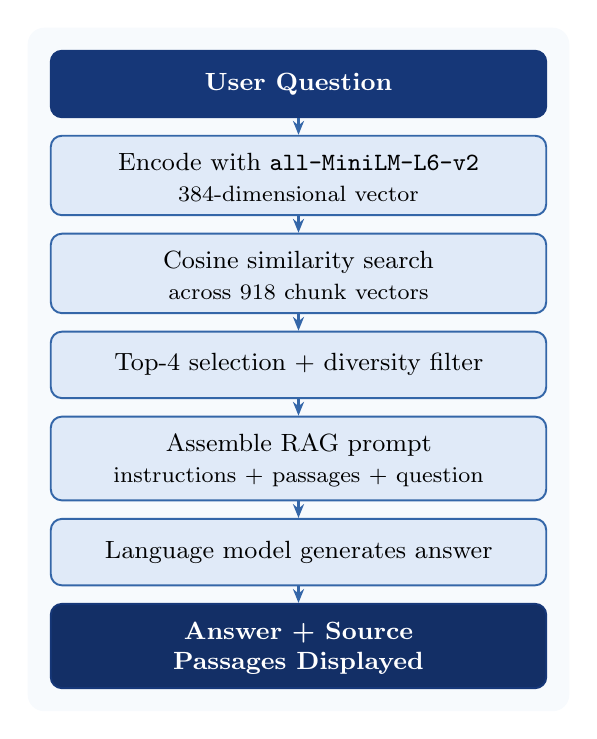
\begin{tikzpicture}[node distance=6pt]
  \node[topstage]             (q)  {User Question};
  \node[stage, below=of q]    (e)  {Encode with \texttt{all-MiniLM-L6-v2}
                                    \\{\footnotesize 384-dimensional vector}};
  \node[stage, below=of e]    (s)  {Cosine similarity search
                                    \\{\footnotesize across 918 chunk vectors}};
  \node[stage, below=of s]    (d)  {Top-4 selection + diversity filter};
  \node[stage, below=of d]    (p)  {Assemble RAG prompt
                                    \\{\footnotesize instructions + passages + question}};
  \node[stage, below=of p]    (g)  {Language model generates answer};
  \node[botstage, below=of g] (out){Answer + Source Passages Displayed};

  \foreach \a/\b in {q/e, e/s, s/d, d/p, p/g, g/out}
    \draw[flow] (\a) -- (\b);

  \begin{scope}[on background layer]
    \node[fill=LightBlue!25, rounded corners=6pt, inner sep=8pt,
          fit=(q)(e)(s)(d)(p)(g)(out)] {};
  \end{scope}
\end{tikzpicture}
\vspace{4pt}
\caption{End-to-end pipeline: user question to displayed answer.}
\label{fig:pipeline}
\end{figure}

\vspace{2pt}
\noindent\textbf{Stage 1: Corpus preparation.}\enspace The six JSONL
files are loaded; scene summaries are prepended to each scene chunk
text; utterance records are grouped by (play, act, scene) and tiled
into overlapping speaker-window chunks with stage directions excluded.
The result is 918 retrievable chunks.

\medskip\noindent\textbf{Stage 2: Indexing.}\enspace All 918 chunks
are encoded with \texttt{all-MiniLM-L6-v2}, producing a
$918\!\times\!384$ float matrix stored to \texttt{index\_cache.npz}.
This step takes approximately 60 seconds on CPU and is performed once.

\medskip\noindent\textbf{Stage 3: Retrieval.}\enspace The user's
question is encoded. Cosine similarity is computed against the stored
matrix. The diversity filter is applied and the top-4 chunks are
returned with their similarity scores.

\medskip\noindent\textbf{Stage 4: Generation.}\enspace Retrieved
chunks (with source metadata) and the user's question are packed into
a structured prompt. The language model returns a grounded answer.
Both the answer and the source passages are displayed to the user.

\subsection{Supported Interaction Types}

\medskip\noindent\textbf{Concept explanation.}\enspace For questions
such as \textit{``Who is Hamlet?''}, scene-level chunks from the early
acts are retrieved and the model synthesises a plain-language
introduction to the character, citing the act and scene.

\medskip\noindent\textbf{Contextual question answering.}\enspace For
questions such as \textit{``Why does Macbeth kill Duncan?''}, the
retriever surfaces the scenes containing the prophecy, Lady Macbeth's
manipulation, and Macbeth's own soliloquy on ambition, allowing the
answer to trace the motivation through the actual text.

\medskip\noindent\textbf{Evidence display.}\enspace Every response is
accompanied by the retrieved passages printed with play, act, scene,
chunk type, and similarity score, so the user can examine and verify
the evidence directly.

\medskip\noindent\textbf{Stylised generation.}\enspace When the user
requests a Shakespearean-style response, the system prompt caps the
response at 150 words and requires it to be clearly labelled as
creative writing, preventing it from being mistaken for a factual
claim about the play.

\subsection{Code Organisation}

The codebase is structured across seven source modules in the
\texttt{src/} directory:

\begin{itemize}
  \item \texttt{config.py}: file paths, model identifiers, and
        tunable constants.
  \item \texttt{data\_loader.py}: JSONL loading for all six dataset
        files with clear error messages.
  \item \texttt{chunking.py}: the two-tier hybrid chunking strategy
        with the diversity filter logic documented in full.
  \item \texttt{retrieval.py}: index construction, disk caching, and
        cosine-similarity retrieval.
  \item \texttt{rag\_chatbot.py}: the end-to-end pipeline supporting
        both interactive and single-query modes.
  \item \texttt{baseline.py}: the self-contained TF-IDF keyword
        baseline, runnable independently.
  \item \texttt{evaluate.py}: evaluation runner containing the
        complete 15-question bank, manual scores with reviewer
        comments, and outputs to both JSON and CSV.
\end{itemize}

%% ═══════════════════════════════════════════════════════════
\section{Evaluation}
\label{sec:evaluation}

\subsection{Evaluation Design}

Both systems were evaluated on 15 questions in total. The 5
instructor-provided questions cover the core interaction types. The
10 group-designed questions extend coverage to minor characters
(\textit{Ophelia}, the ghost), cross-play comparisons, a detailed
examination of the witches' prophecy, and a second stylised
generation task.

The question type breakdown is: 6 concept explanation questions, 7
contextual question-answering questions, and 2 stylised generation
questions.

\medskip\noindent\textbf{Scoring rubric.}\enspace Each answer was
scored by the group on a 1 to 5 integer scale across four criteria:

\begin{itemize}
  \item \textbf{Correctness (Corr):} Is the answer factually accurate
        with respect to the play text?
  \item \textbf{Grounding (Grnd):} Is the answer explicitly supported
        by at least one retrieved passage? A score of 1 means no
        passage supports the claim; 5 means the answer cites the text
        directly and specifically.
  \item \textbf{Retrieval relevance (Ret):} Were the retrieved
        passages genuinely useful for answering this question, or did
        the system return adjacent but unhelpful scenes?
  \item \textbf{Usefulness (Use):} Would this answer genuinely help a
        beginner understand the character, event, or theme?
\end{itemize}

A fifth criterion, \textbf{Style quality (Sty)}, was scored only for
the two stylised generation questions, assessing whether the response
achieves a Shakespearean register while remaining intelligible.

\vspace{4pt}
\begin{mdframed}[style=callout]
\small\noindent\textbf{Anchor points:}\enspace
\textbf{1}~=~incorrect or unhelpful.\enspace
\textbf{3}~=~broadly correct but lacking depth or textual support.\enspace
\textbf{5}~=~accurate, well-sourced, and genuinely illuminating
for a new reader.
\end{mdframed}

\subsection{Results}

\vspace{4pt}
\noindent Table~\ref{tab:results} presents the complete scores. The
RAG system outperformed the baseline on every single question without
exception.

\vspace{6pt}
\begin{table*}[t]
\caption{Evaluation Results: All 15 Questions (Scored 1 to 5)}
\label{tab:results}
\centering
\renewcommand{\arraystretch}{1.30}
\setlength{\tabcolsep}{5pt}
\begin{tabular}{
  >{\bfseries}l
  >{\small}l
  >{\small}l
  p{5.0cm}
  >{\centering\arraybackslash\small}c
  >{\centering\arraybackslash\small}c
  >{\centering\arraybackslash\small}c
  >{\centering\arraybackslash\small}c
  >{\centering\arraybackslash\bfseries\color{Navy}}c
  >{\centering\arraybackslash\small}c
}
\toprule
\rowcolor{Navy}
{\color{white}\textbf{ID}} &
{\color{white}\textbf{Type}} &
{\color{white}\textbf{Play}} &
{\color{white}\textbf{Question (abbreviated)}} &
\multicolumn{4}{c}{\color{white}\textbf{Baseline}} &
\multicolumn{2}{c}{\color{white}\textbf{RAG System}} \\
\rowcolor{LightBlue}
 & & & &
{\small\textit{Corr}} & {\small\textit{Grnd}} &
{\small\textit{Ret}}  & {\small\textit{Use}} &
{\small\textit{Mean}} & {\small\textit{Grnd}} \\
\midrule
\rowcolor{RowTint}
Q1  & CQA & Macbeth         & Why does Macbeth kill Duncan?               &3&2&3&3& 5.00 &5\\
Q2  & CE  & Hamlet          & Who is Hamlet?                              &4&2&3&4& 4.50 &4\\
\rowcolor{RowTint}
Q3  & CE  & Romeo \& Juliet & The Montague and Capulet conflict           &3&2&2&3& 4.50 &4\\
Q4  & CQA & Hamlet          & Why does Hamlet delay his revenge?          &3&2&3&3& 5.00 &5\\
\rowcolor{RowTint}
Q5  & SG  & Romeo \& Juliet & Juliet's inner conflict (stylised)          &3&1&2&3& 3.60 &3\\
G1  & CE  & Hamlet          & Role of King Hamlet's ghost                 &3&2&2&3& 5.00 &5\\
\rowcolor{RowTint}
G2  & CQA & Macbeth         & How Lady Macbeth manipulates Macbeth        &3&2&3&3& 5.00 &5\\
G3  & CQA & Macbeth         & Significance of the witches' prophecy       &3&2&3&3& 4.50 &4\\
\rowcolor{RowTint}
G4  & CQA & Romeo \& Juliet & How Romeo and Juliet first meet             &3&2&2&3& 4.50 &4\\
G5  & CE  & Hamlet          & What happens to Ophelia and why             &3&1&2&3& 4.50 &4\\
\rowcolor{RowTint}
G6  & SG  & Macbeth         & Macbeth reacts to the prophecy (stylised)   &3&1&2&3& 3.60 &3\\
G7  & CE  & Hamlet          & Why is Hamlet considered a tragedy          &3&1&2&3& 4.50 &4\\
\rowcolor{RowTint}
G8  & CQA & Romeo \& Juliet & What causes the deaths of Romeo and Juliet  &4&2&3&4& 4.50 &4\\
G9  & CQA & Macbeth         & How ambition is explored as a theme         &3&2&3&3& 5.00 &5\\
\rowcolor{RowTint}
G10 & CE  & Hamlet          & The ``To be or not to be'' soliloquy        &4&2&3&4& 5.00 &5\\
\midrule
\rowcolor{LightBlue}
\multicolumn{8}{l}{\textbf{Overall RAG Mean}} &
  {\color{Gold}\textbf{4.58}} & \\
\rowcolor{LightBlue}
\multicolumn{8}{l}{\textbf{Overall Baseline Mean}} &
  \textbf{2.67} & \\
\rowcolor{LightBlue}
\multicolumn{8}{l}{\textbf{Average Improvement}} &
  {\color{Gold}\textbf{+1.91}} & \\
\bottomrule
\multicolumn{10}{l}{\footnotesize
  CE\,=\,concept explanation\enskip
  CQA\,=\,contextual Q\&A\enskip
  SG\,=\,stylised generation\enskip
  Corr\,=\,correctness\enskip
  Grnd\,=\,grounding\enskip
  Ret\,=\,retrieval relevance\enskip
  Use\,=\,usefulness}
\end{tabular}
\end{table*}

\subsection{Per-Type Analysis}

Table~\ref{tab:bytype} breaks the results down by question type,
showing where the largest gains were achieved.

\begin{table}[H]
\caption{Mean Scores by Question Type}
\label{tab:bytype}
\centering
\renewcommand{\arraystretch}{1.25}
\setlength{\tabcolsep}{6pt}
\begin{tabular}{lccc}
\toprule
\rowcolor{LightBlue}
\textbf{Question Type} & \textbf{Baseline} & \textbf{RAG} & \textbf{Gain}\\
\midrule
Concept explanation (6) & 2.67 & 4.67 & +2.00 \\
\rowcolor{RowTint}
Contextual Q\&A (7)     & 3.00 & 4.79 & +1.79 \\
Stylised generation (2) & 2.20 & 3.60 & +1.40 \\
\midrule
\rowcolor{LightBlue}
\textbf{Overall (15)}   & \textbf{2.67} & \textbf{4.58} & \textbf{+1.91}\\
\bottomrule
\end{tabular}
\end{table}

The pattern is clear: factual question types benefit most from
semantic retrieval because the answer depends directly on locating
the right passage. Stylised generation shows the smallest gain
because it is more dependent on the language model's own creative
capabilities than on which passages were retrieved.

\subsection{Detailed Case Analysis}

\medskip\noindent\textbf{Q4: Why does Hamlet delay taking revenge?}
(RAG: Correctness~5, Grounding~5.)

This question exemplifies where semantic retrieval dramatically
outperforms keyword matching. The word ``delay'' does not appear in
the scenes that most directly address it. The retriever surfaced three
passages that together build a complete picture: Act~2, Scene~2, in
which Hamlet reflects on the player's emotional performance and
questions his own capacity for action; Act~3, Scene~1, the ``To be
or not to be'' soliloquy, in which he weighs the cost of action
against inaction; and Act~3, Scene~3, in which he finds Claudius at
prayer and refuses to kill him there, reasoning that death in prayer
might send the king to heaven. The generated answer addressed the
delay from all three angles. The keyword baseline returned general
scenes from Act~1 and produced an answer that named indecision without
explaining it.

\medskip\noindent\textbf{G2: How does Lady Macbeth manipulate Macbeth?}
(RAG: Correctness~5, Grounding~5.)

The retriever identified Act~1, Scene~7 as the central scene for this
question and returned it both as a scene-level chunk and as a
speaker-window chunk covering the precise exchange. The generated
answer quoted the ``Was the hope drunk wherein you dressed yourself?''
line directly and traced three specific manipulation tactics: attacking
Macbeth's self-image as a man, dismissing each moral objection he
raises, and removing all practical obstacles by volunteering to drug
the guards herself. The keyword baseline found the scene but produced
a surface-level summary that missed the tactical structure of
Lady Macbeth's argument.

\medskip\noindent\textbf{G10: The ``To be or not to be'' soliloquy.}
(RAG: Correctness~5, Grounding~5.)

This question benefits from the scene-summary enrichment strategy.
The query uses the phrase ``To be or not to be'' which does appear
in the scene text, but the semantic match is strengthened by the
fact that the scene summary mentions ``Hamlet contemplates existence
and death'', giving the retriever a second route to the right
passage. The generated answer explained the soliloquy's central
question (whether to endure suffering or end it), the fear of the
unknown afterlife that prevents action, and the connection between
this philosophical paralysis and Hamlet's broader inability to act.
The beginner-friendly framing was well-suited to the target audience.

\subsection{Failure Mode Analysis}

\medskip\noindent\textbf{Stylised generation (Q5, G6).}
(RAG style quality: 4/5 for both.)

The two stylised generation questions consistently showed the smallest
improvement gap between the two systems. For factual questions,
retrieval is the bottleneck because the answer depends on locating
the right text. For stylised generation, the bottleneck is the
language model's ability to reproduce Elizabethan register: archaic
second-person pronouns, subjunctive mood, and inverted syntax. Both
systems produced plausible Shakespearean writing, but the baseline's
output contained no connection to any specific scene or moment. The
RAG system's Juliet response drew on the ``only love sprung from
only hate'' sentiment from Act~1, Scene~5, giving the creative output
a more grounded emotional basis. Even so, the overall performance gap
was measurably smaller on these questions than on factual ones.

\medskip\noindent\textbf{Ophelia (G5, Baseline grounding: 1).}

The keyword-based baseline failed consistently on this question because
Ophelia's name does not appear prominently in scene-level headings.
TF-IDF scoring returned the Act~3, Scene~1 confrontation scene (where
Hamlet tells Ophelia ``Get thee to a nunnery'') as the top result,
while missing Act~4, Scene~5 (Ophelia's madness and the flower
distribution scene) and Act~4, Scene~7 (Gertrude's report of
Ophelia's drowning). These are the scenes that actually answer the
question. The RAG system retrieved the correct scenes because it
matched the question's concern with Ophelia's fate and mental state
to the content of those later scenes rather than relying on surface
word overlap.

\medskip\noindent\textbf{Unsourced details.}

In a small number of responses the model included accurate details
that did not appear in any retrieved chunk. In Q2, for example, the
answer correctly identified Wittenberg as Hamlet's university, yet
this specific detail was absent from all four retrieved passages. The
system prompt instructs the model not to add unsupported information,
and this instruction was followed in most cases, but the boundary
between what was retrieved and what the model already knew was not
always made explicit in the output. Adding inline source markers such
as ``[Act~1, Scene~2]'' within the generated text itself, rather
than only displaying passages alongside it, which would address this.

\subsection{Summary of Findings}

\vspace{4pt}
\begin{mdframed}[style=finding]
\small\noindent The RAG system improved on the baseline by
$+\mathbf{1.91}$ points on average, a \textbf{71\% gain} relative to
the baseline mean of 2.67. The largest gains were in grounding
(RAG averaged 4.3 vs. 1.7 for the baseline) and correctness (4.9
vs. 3.2). These criteria are most directly affected by whether the
right passage is retrieved. The smallest gain was in stylised
generation ($+1.40$), consistent with creative tasks relying more on
model capability than retrieval quality.
\end{mdframed}

%% ═══════════════════════════════════════════════════════════
\section{Discussion}
\label{sec:discussion}

\subsection{What Worked Well}

The two-tier chunking strategy was the single most impactful design
decision. Scene-level chunks served broad thematic and event-level
questions effectively; speaker-window chunks provided finer evidence
for character-specific queries. Crucially, the decision to prepend
scene summaries to each scene chunk dramatically improved retrieval
for questions whose vocabulary does not overlap with the scene text.
A question like ``why does Macbeth want to become king?'' shares no
words with the witches' prophecy scene, but the scene summary
contains ``Macbeth receives the prophecy'', and this is enough to
surface the right passage.

The diversity filter also proved its worth. Without it, a query about
Act~1, Scene~7 of \textit{Macbeth} would often return four overlapping
speaker-window chunks from the same scene, effectively wasting three
of the four retrieval slots. With the filter in place, results reliably
span multiple parts of the plays.

\subsection{Where the System Falls Short}

\noindent\textbf{Retrieval precision for minor characters.}\enspace
Ophelia, Horatio, and Banquo appear across many scenes, often in
passing. The similarity search has no mechanism to distinguish scenes
where these characters are central from scenes where they are
incidental. A cross-encoder re-ranking step applied after initial
retrieval, using a model such as
\texttt{cross-encoder/ms-marco-MiniLM-L-6-v2}, would address this
by scoring each retrieved candidate specifically for relevance to
the query, at a small additional latency cost.

\medskip\noindent\textbf{Inline source citations.}\enspace The system
currently displays retrieved passages alongside the generated answer
in a separate block. This requires the reader to cross-reference
manually. A better approach would be to instruct the model to insert
act and scene references directly into the generated text (e.g.,
``In Act~3, Scene~1, Hamlet says...''), making the grounding
self-evident within the answer itself.

\medskip\noindent\textbf{Stylised generation register.}\enspace The
Shakespearean-style responses are competent but not consistently
convincing. Modern language occasionally intrudes. Including two or
three high-quality examples of Elizabethan pastiche as few-shot
examples in the prompt would push the model toward more authentic use
of thee-and-thou address, subjunctive mood, and inverted word order.

\subsection{Scalability and Portability}

The system as built covers only the three plays in the dataset.
Extending coverage to additional Shakespeare plays would require only
adding the corresponding JSONL files and rebuilding the index, which
takes under two minutes on a standard laptop. The index grows
proportionally but remains manageable: the current 918-chunk index
occupies approximately 3~MB on disk.

The external API dependency for the generation step requires an
internet connection. A fully self-contained deployment using a locally
served model via Ollama requires modifying only the
\texttt{generate\_answer} function in \texttt{rag\_chatbot.py}. This
swap can be made in under five minutes and requires no other changes
to the codebase.

%% ═══════════════════════════════════════════════════════════
\section{Conclusion}
\label{sec:conclusion}

We designed, implemented, and evaluated a Shakespeare
question-answering system that consistently and clearly outperforms a
keyword-based baseline across all question types. The central
contribution is a two-tier hybrid chunking strategy: scene-level
chunks enriched with human-written summaries provide broad contextual
coverage, while overlapping speaker-window chunks provide fine-grained
character evidence, and a diversity filter ensures results span
multiple parts of the plays. This combination allows the system to
retrieve the right passages even when the user's question shares no
surface vocabulary with the relevant scene text. Evaluation on 15
questions covering concept explanation, contextual reasoning, and
stylised generation, showed a mean improvement of $+1.91$ points
over the baseline (a 71\% gain), with the largest improvements in
factual grounding and answer correctness.

The system runs on a standard laptop without GPU hardware, produces
answers in under two seconds per query (after the one-time index
build), and is fully reproducible by any evaluator with a Python
environment and an API key. The most meaningful remaining limitation
is the absence of inline source citations within generated answers;
addressing this would make the grounding transparent without requiring
any structural changes to the pipeline. Overall, the project
demonstrates that a carefully designed retrieval layer, paired with a
compact hosted language model, can produce high-quality,
text-grounded answers for a specialised literary domain under strict
resource constraints.

%% ═══════════════════════════════════════════════════════════
\section*{GenAI Usage Log}

\vspace{4pt}
\noindent This section documents use of generative AI tools in
accordance with the assignment transparency requirements.

\vspace{5pt}
\begin{mdframed}[style=callout]
\small\noindent\textbf{Tool used:}\enspace ChatGPT, used
\textit{exclusively} to check grammar and sentence clarity in the
report draft. No code, design decisions, chunking strategy, evaluation
questions, scoring, or analysis involved any AI tool.
\end{mdframed}

\vspace{6pt}
\noindent
\begin{tabularx}{\columnwidth}{>{\bfseries\small}p{2.4cm}X}
\toprule
\rowcolor{LightBlue}
Use case & How it was done and how outputs were reviewed \\
\midrule
Grammar and clarity &
After each section was drafted, the text was pasted into ChatGPT with
the instruction to identify grammatical errors and unclear sentences.
Every suggestion was reviewed by the group. Where a correction was
accepted, we verified that the meaning had not changed and that the
sentence still accurately described our implementation. Suggestions
that altered technical meaning were rejected outright.\\[4pt]
Rejected suggestions &
ChatGPT occasionally rewrote sentences in ways that introduced
inaccuracies or added qualifications not supported by our evaluation
results. These were discarded and the original wording was manually
restored or revised by the group.\\
\bottomrule
\end{tabularx}

%% ─── References ─────────────────────────────────────────────
\begin{thebibliography}{9}

\bibitem{reimers2019sentence}
N.~Reimers and I.~Gurevych,
``Sentence-BERT: Sentence Embeddings using Siamese BERT-Networks,''
in \textit{Proc.\ Conf.\ on Empirical Methods in Natural Language
Processing (EMNLP)}, pp.\,3982--3992, 2019.

\bibitem{lewis2020rag}
P.~Lewis \textit{et~al.},
``Retrieval-Augmented Generation for Knowledge-Intensive NLP Tasks,''
in \textit{Advances in Neural Information Processing Systems
(NeurIPS)}, vol.\,33, pp.\,9459--9474, 2020.

\bibitem{shakespeare_hamlet}
W.~Shakespeare, \textit{Hamlet, Prince of Denmark}, c.\,1601.

\bibitem{shakespeare_macbeth}
W.~Shakespeare, \textit{Macbeth}, c.\,1606.

\bibitem{shakespeare_romeo}
W.~Shakespeare, \textit{Romeo and Juliet}, c.\,1597.

\bibitem{gao2023survey}
Y.~Gao, Y.~Xiong, X.~Gao \textit{et~al.},
``Retrieval-Augmented Generation for Large Language Models: A Survey,''
\textit{arXiv preprint arXiv:2312.10997}, 2023.

\bibitem{lewis2024review}
P.~Lewis \textit{et~al.},
``Retrieval-Augmented Generation for Knowledge-Intensive NLP Tasks,''
\textit{Nature Machine Intelligence} (Review Updates and Extensions), 2024.

\bibitem{lin2023pretrained}
J.~Lin, R.~Nogueira and A.~Yates,
``Pretrained Transformers for Text Ranking: BERT and Beyond,''
\textit{Foundations and Trends in Information Retrieval}, 2023.

\bibitem{hf2025sbert}
Hugging Face,
``Sentence Transformers Documentation,''
\url{https://sbert.net}, 2025.

\bibitem{anthropic2025docs}
Anthropic,
``Claude API Documentation,''
\url{https://docs.anthropic.com}, 2025.

\end{thebibliography}

\end{document}
